\section{Ablation Studies}
\label{sec:appendix_ablations}

\vspace{-0.25em}
\noindent
This appendix isolates \textbf{which components actually matter} for SwiPO and \textbf{why}.
Our central hypothesis is that SwiPO succeeds at \textbf{instruction-conditioned switching} only when the optimization remains within a \textbf{stable local neighborhood} of a reference policy while still learning \textbf{sharp, instruction-dependent preference gaps}.
Accordingly, we ablate the two parameters that directly control this trade-off:
\textbf{(i) the KL anchor weight} $\lambda_{\text{KL}}$, which governs \textbf{stability and regime co-existence}, and
\textbf{(ii) the preference temperature} $\beta$, which governs \textbf{gap sharpness and switching sensitivity}.
We report three outcome signals throughout:
\textbf{reward margin} (training separation), \textbf{ECLIPTICA score} (switchability under controlled instruction flips), and \textbf{stability} (run-to-run and within-run behavior).

% -----------------------------------------------------------------------------
% KL-weight and beta ablation subsections removed 2026-10-20: no such runs exist (the trainer rejects
% lambda_KL <= 0 and Optuna sampled beta only in [0.08, 0.15]); see ARR_feedback/audit_v5_discrepancy.md rows 17-18.

\subsection{Hyperparameter Sensitivity (Optuna/TPE)}
% -----------------------------------------------------------------------------

\vspace{-0.25em}
\noindent
We run 13 Optuna trials with TPE sampling for SwiPO\_Instruct.
TPE proposes configurations by fitting densities over \textbf{good} vs.\ \textbf{bad} trials and sampling where expected improvement is highest.
We optimize learning rate, weight decay, $\beta$, and $\lambda_{\text{KL}}$.
Figure~\ref{fig:hp_ablation_combined} summarizes the sensitivity of reward margin to these hyperparameters, revealing a concentrated ``good'' region rather than a broad plateau.

\begin{figure*}[p]
\centering
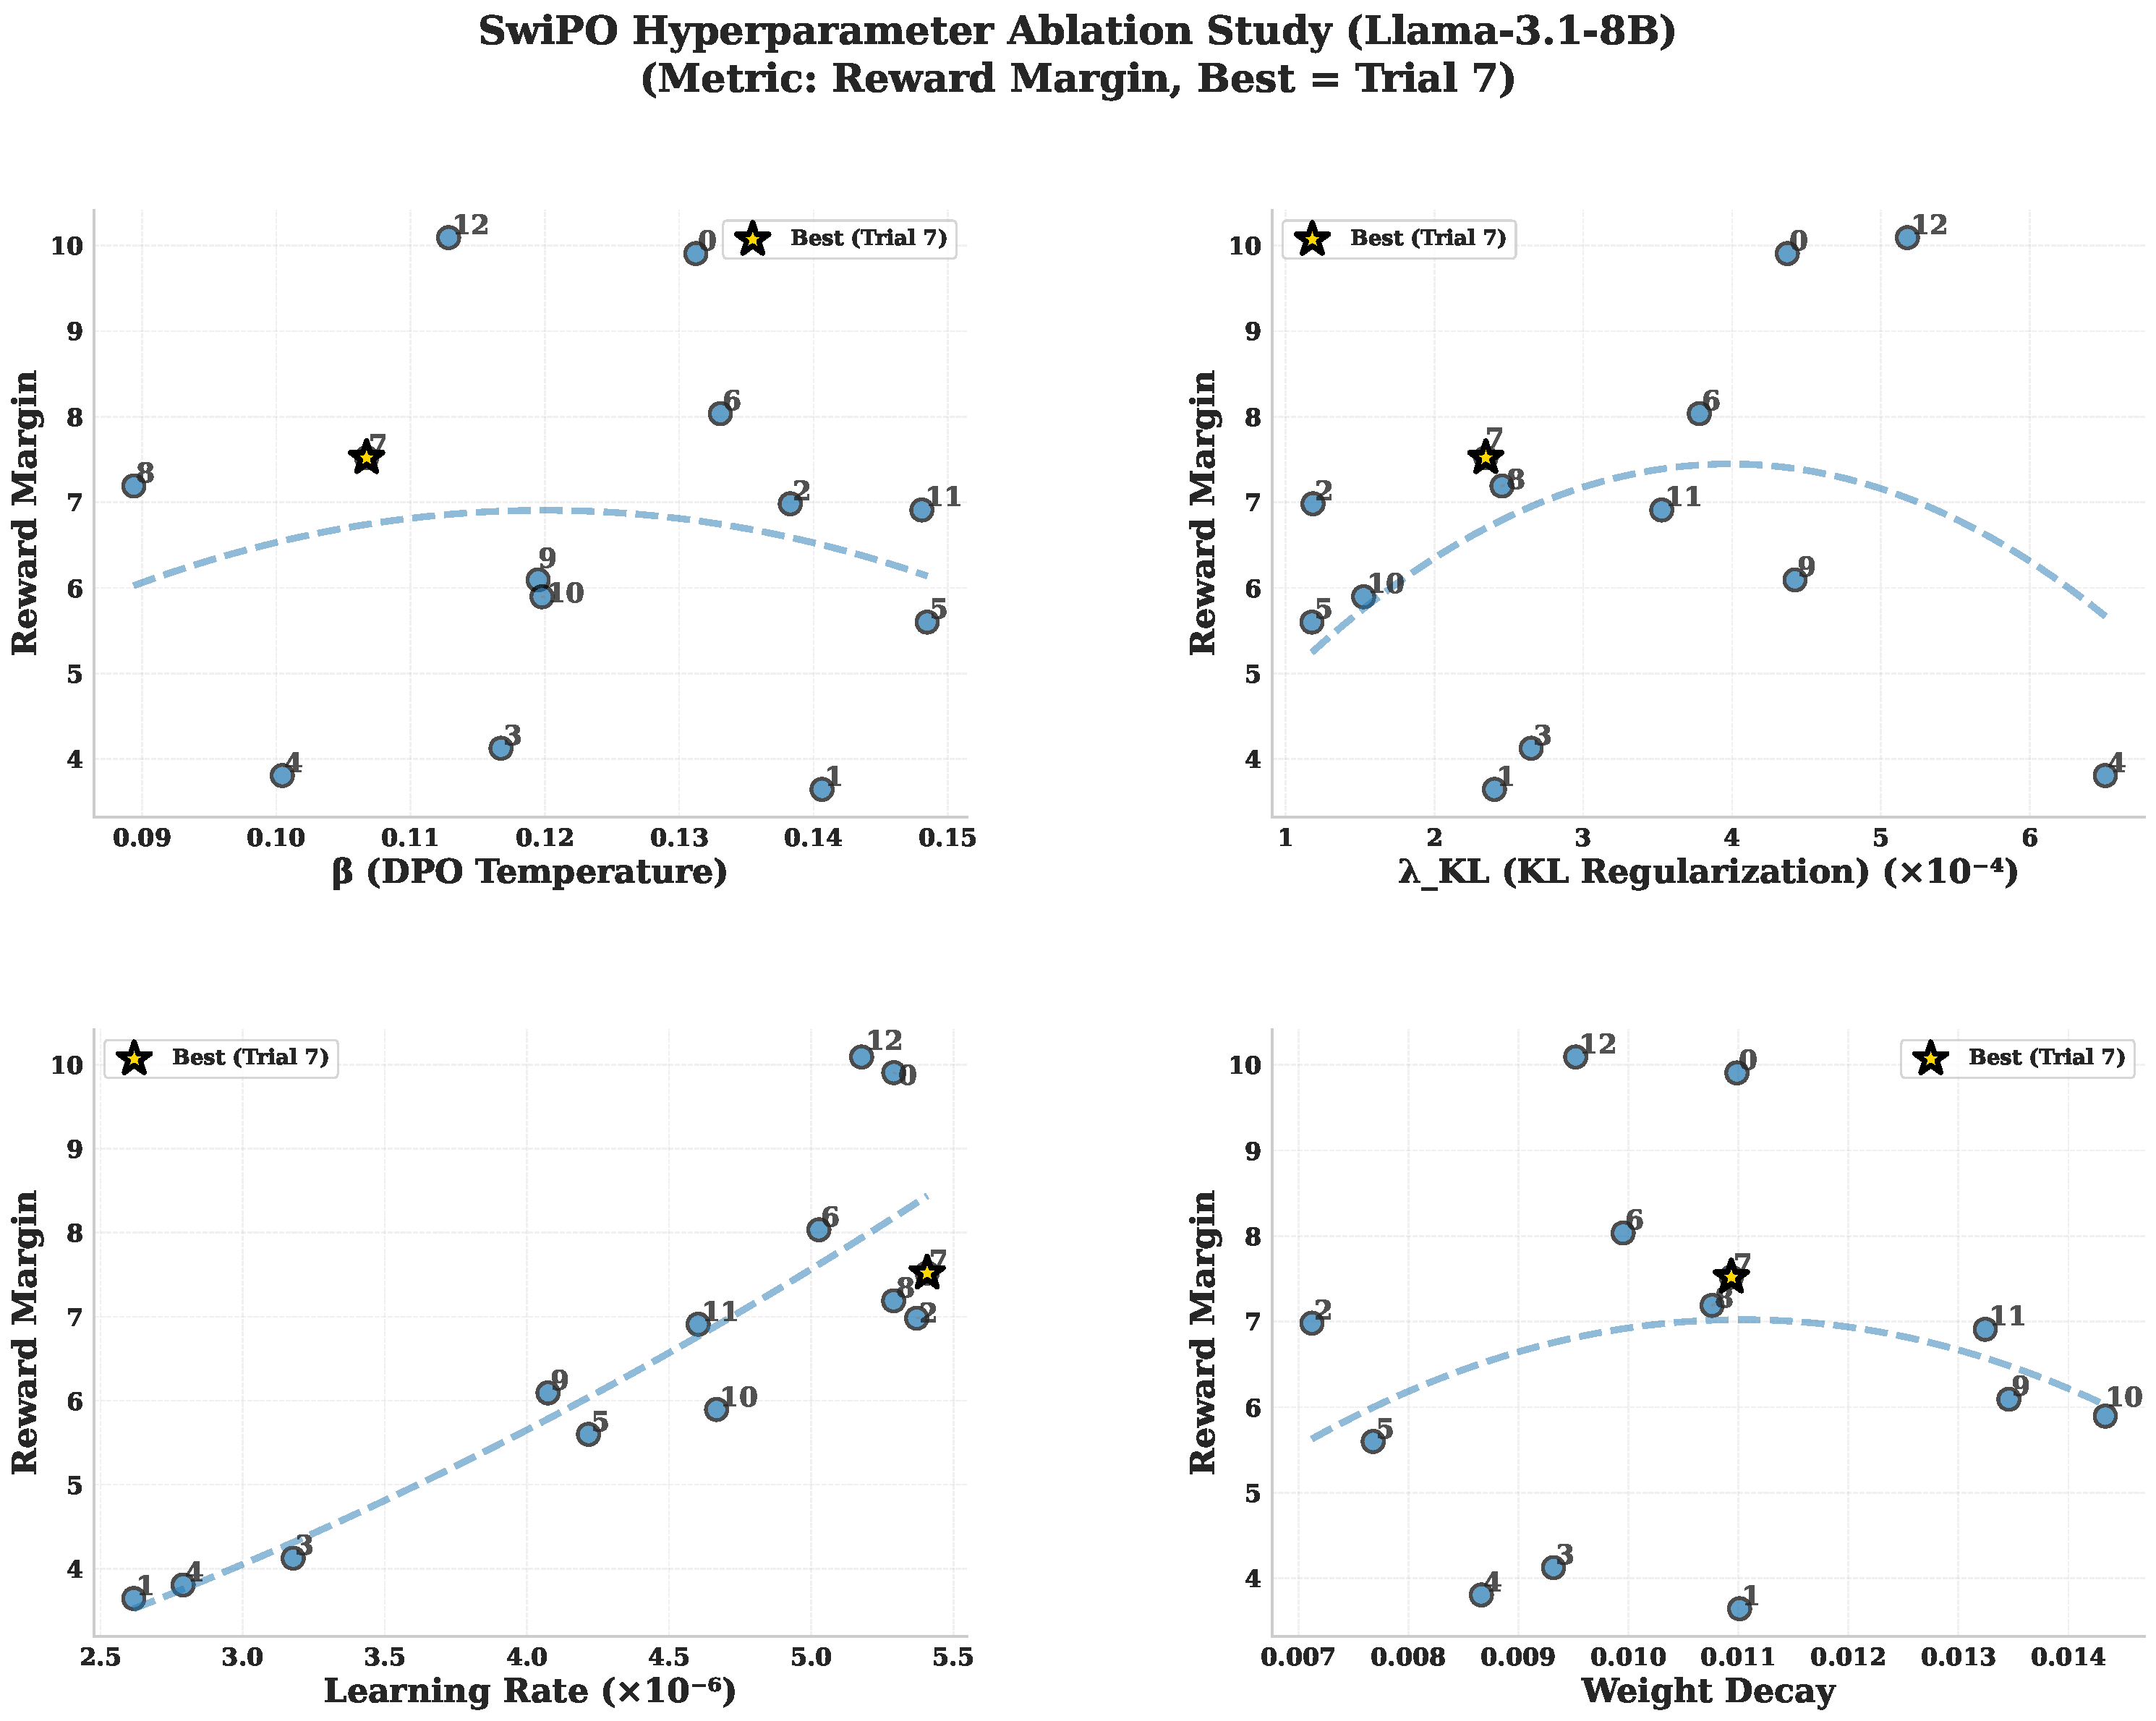
\includegraphics[width=0.85\textwidth]{figures/appendix/hp_ablation_combined.pdf}
\caption{\textbf{Hyperparameter sensitivity across 13 Optuna trials.} Reward margin is most sensitive to learning rate and the $(\beta,\lambda_{\text{KL}})$ interaction. Trial 7 ($\star$) achieves the best trade-off, aligning with the ``Goldilocks'' band: $\beta\in[0.10,0.12]$, $\lambda_{\text{KL}}\approx 2\times 10^{-4}$, and LR $\approx 5\times 10^{-6}$.}
\label{fig:hp_ablation_combined}
\end{figure*}

\paragraph{Reading the 4-panel ablation.}
Figure~\ref{fig:hp_ablation_combined} presents reward margin (y-axis) against each of the four tuned hyperparameters (x-axis): $\beta$ (DPO temperature), $\lambda_{\text{KL}}$ (KL regularization coefficient), learning rate, and weight decay.
Each blue point represents one of 13 Optuna trials, with Trial 7 ($\star$) highlighted as the best configuration.
Dashed trend lines (polynomial fits) reveal the functional relationship between each hyperparameter and reward margin.
The key observation is that reward margin is \textbf{not uniformly sensitive} to all hyperparameters: learning rate shows a strong positive correlation (higher LR $\rightarrow$ higher margin up to a point), while weight decay shows weaker sensitivity with high variance.

\paragraph{Identifying the ``Goldilocks zone''.}
Across all four panels, Trial 7 consistently appears near the peak of the trend curve, confirming that the selected configuration occupies the \textbf{intersection of optimal regions} across hyperparameters.
The $\beta$ panel shows a peaked distribution with optimum around 0.10--0.12; the $\lambda_{\text{KL}}$ panel shows an inverted-U with optimum around $2$--$3 \times 10^{-4}$; the learning rate panel shows monotonic increase up to $\sim 5 \times 10^{-6}$; and the weight decay panel shows weak sensitivity.
This multi-dimensional view explains why naive grid search would be inefficient: the optimal region is a narrow \textbf{tube} in 4D space, not a hyperrectangle.

\paragraph{Why TPE sampling works.}
The Tree-structured Parzen Estimator (TPE) searches this space efficiently by modeling $P(\text{hyperparameters} | \text{good})$ vs.\ $P(\text{hyperparameters} | \text{bad})$.
Trials 0--4 explore broadly; trials 5--12 concentrate near promising regions.
The final distribution of points shows TPE's adaptive behavior: dense sampling near $\beta \approx 0.11$, $\lambda_{\text{KL}} \approx 2 \times 10^{-4}$, and LR $\approx 5 \times 10^{-6}$, with sparse exploration of poor regions (low LR, extreme $\beta$).

\vspace{-0.25em}
\noindent
\textbf{Pareto structure.}
Because reward margin and preference accuracy do not perfectly correlate with ECLIPTICA switchability, we additionally analyze margin--accuracy trade-offs.
Figure~\ref{fig:hp_pareto} shows the Pareto frontier; the selected configuration lies on the frontier, indicating that further margin gains typically require accuracy/switchability trade-offs.

\begin{figure}[ht!]
\centering
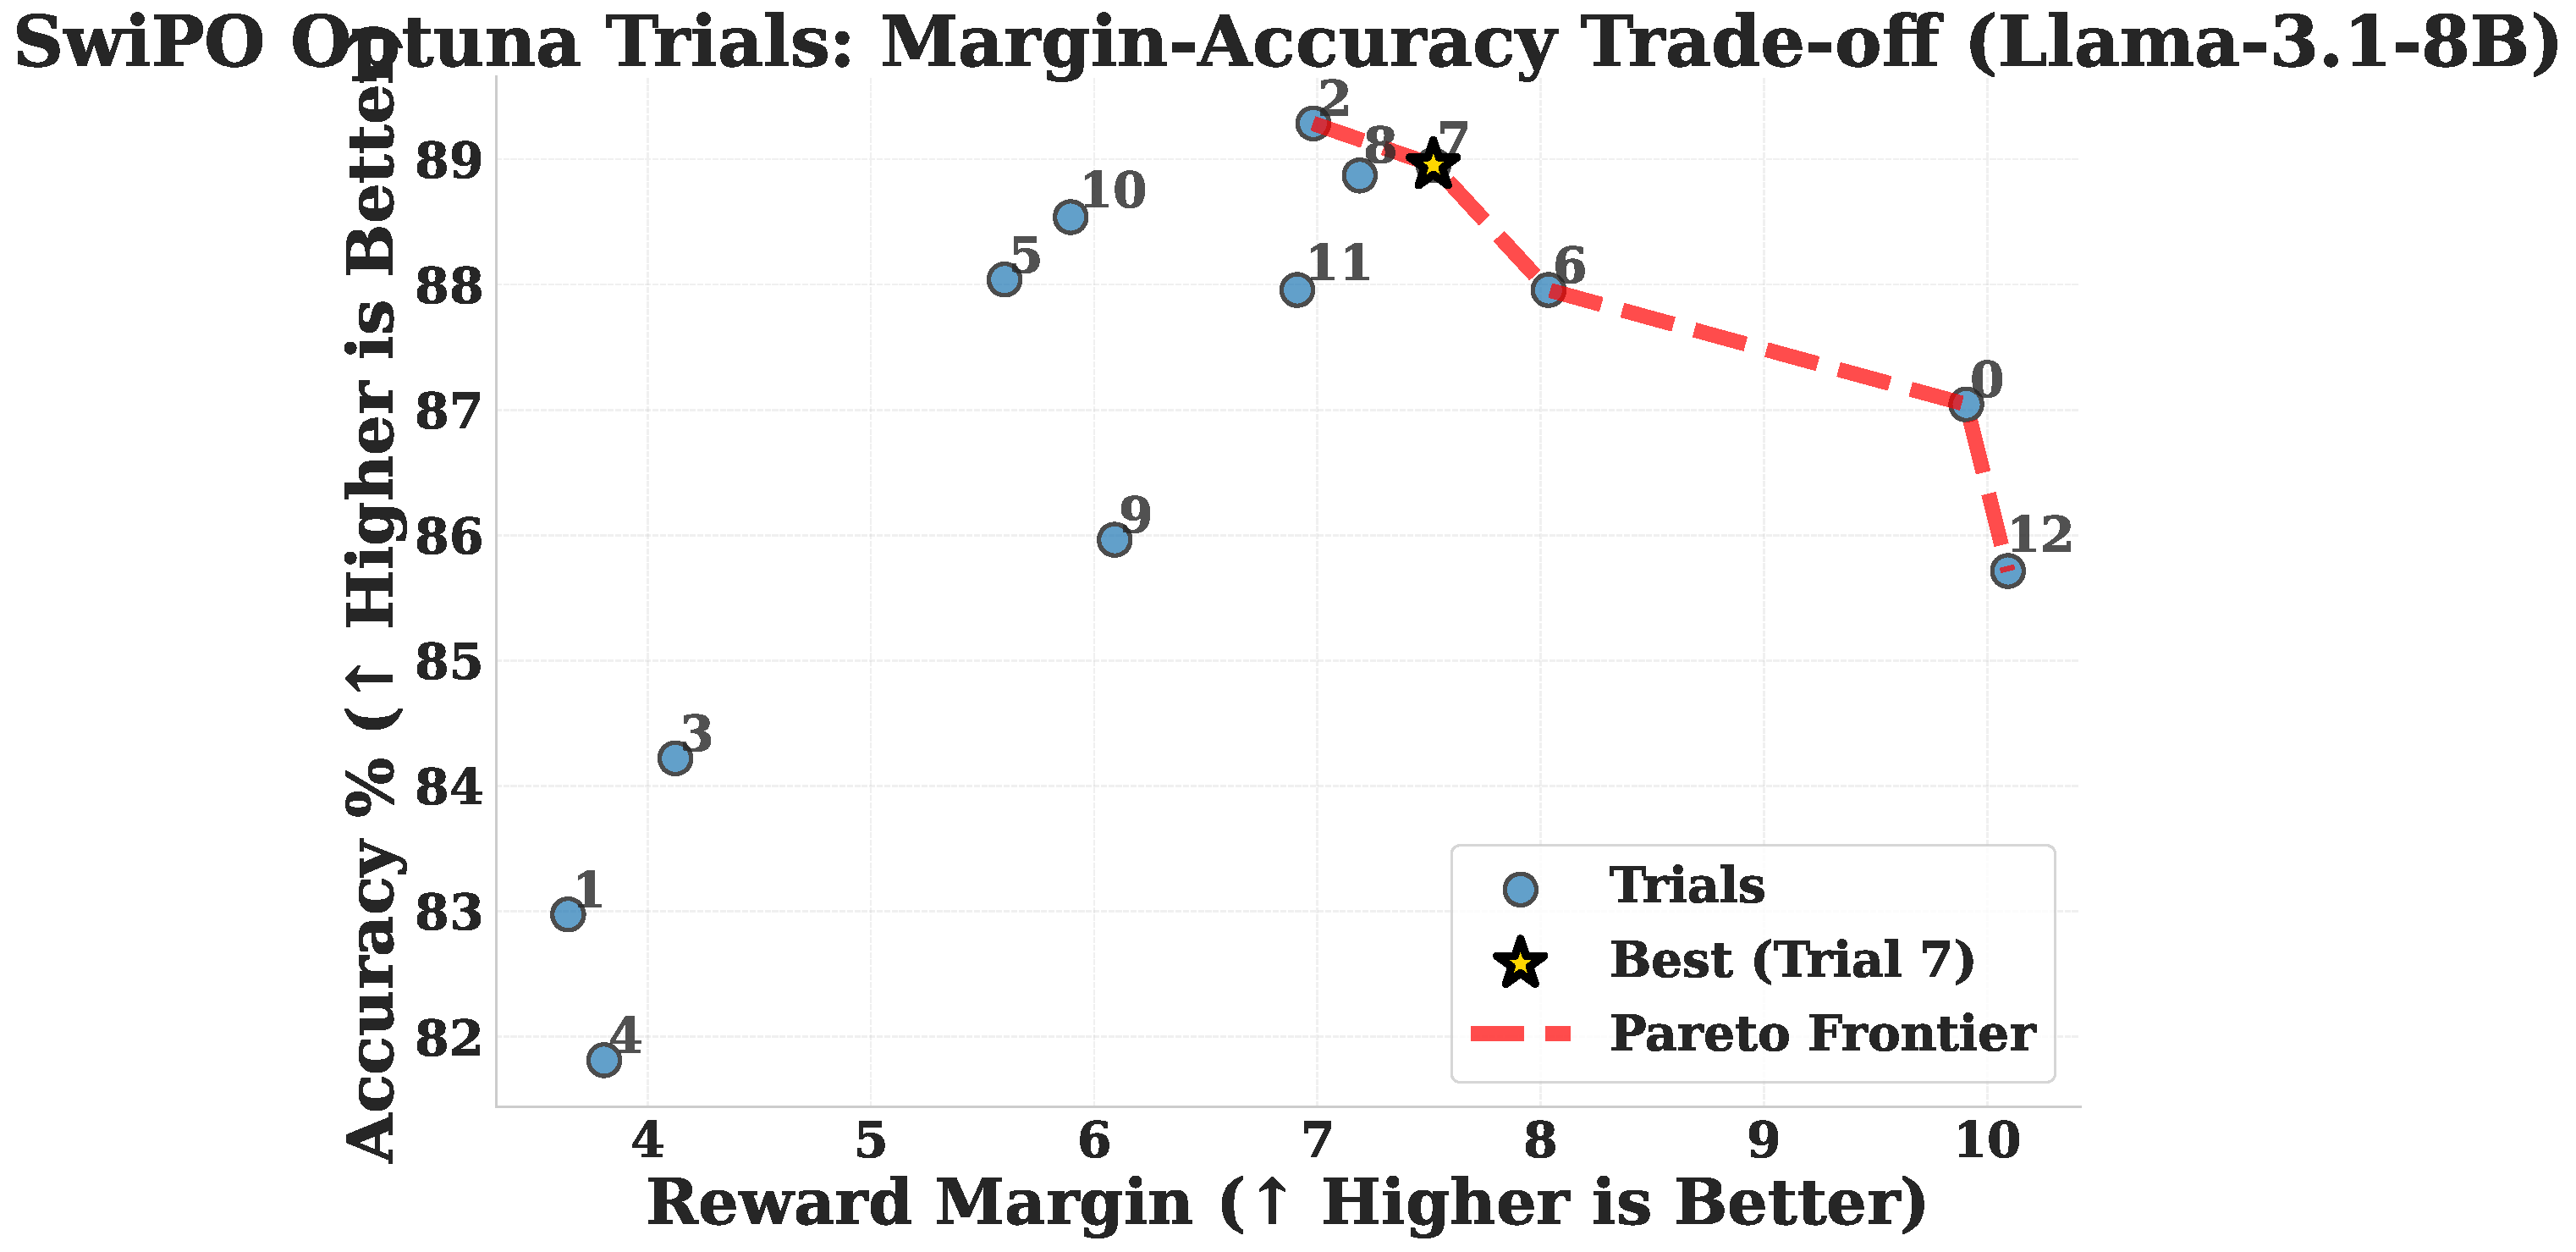
\includegraphics[width=0.9\columnwidth]{figures/appendix/hp_pareto_frontier.pdf}
\caption{\textbf{Pareto frontier across trials.} Trial 7 lies on the frontier, achieving near-optimal balance (margin=7.52, accuracy=89\%) while maintaining strong instruction-conditioned switching.}
\label{fig:hp_pareto}
\end{figure}

\paragraph{Interpreting the Pareto frontier.}
Figure~\ref{fig:hp_pareto} plots the two primary training objectives, reward margin (x-axis, higher is better) and preference accuracy (y-axis, higher is better), for all 13 Optuna trials.
The red dashed line traces the \textbf{Pareto frontier}: configurations where no other trial dominates on both objectives.
Trials below or left of this frontier are Pareto-dominated (another trial is better on at least one axis without being worse on the other).
Among these 13 trials, the two with margin $>$9 (trials 0, 12) have accuracy of $\sim$85--87\%, and the two with accuracy $>$89\% (trials 2, 8) have margins near 7; with one seed per trial this is a pattern in 13 points, not a measured trade-off.

\paragraph{Why Trial 7 is optimal for switching.}
Trial 7 ($\star$) achieves margin 7.52 with accuracy 89\%, placing it \textbf{on the Pareto frontier} at the ``knee'' where both objectives are near-optimal.
Trial 7 was selected on these two training-time objectives. No per-trial ECLIPTICA evaluation was run, so whether the knee also maximizes switching is untested. Trials 0 and 12 reach higher margins (9.9, 10.1) at lower accuracy (87\%, 86\%).

\paragraph{Multi-objective optimization justification.}
This Pareto analysis justifies our multi-objective Optuna formulation (maximize margin, maximize accuracy, minimize eval loss).
Single-objective optimization on margin alone would select trials 0 or 12, at lower preference accuracy.
Selecting at the knee of the frontier keeps both training objectives near their best; its effect on switching was not measured per trial.

\vspace{-0.35em}
\noindent\textbf{Trial 7 analysis (why it wins).}
The best configuration ($\beta$=0.107, $\lambda_{\text{KL}}$=0.00023, LR=5.4e-6) occupies a narrow region where:
\textbf{(i) $\beta$ is high enough} to separate instruction-conditioned preferences,
\textbf{(ii) $\lambda_{\text{KL}}$ is strong enough} to prevent regime drift,
and \textbf{(iii) LR is low enough} to avoid overshooting under longer instruction-augmented sequences.
This ``alignment'' of the three levers yields high margins without sacrificing switchability.

% -----------------------------------------------------------------------------
\subsubsection{Individual Hyperparameter Analysis}
% -----------------------------------------------------------------------------

\vspace{-0.25em}
\noindent
Figures~\ref{fig:hp_beta}--\ref{fig:hp_lr} provide per-parameter sensitivity analyses, plotting reward margin, accuracy, and evaluation loss.
Across plots, Trial 7 ($\star$) consistently appears near the optimal region, indicating that the final choice is not an outlier but a coherent solution across axes.

\begin{figure*}[p]
\centering
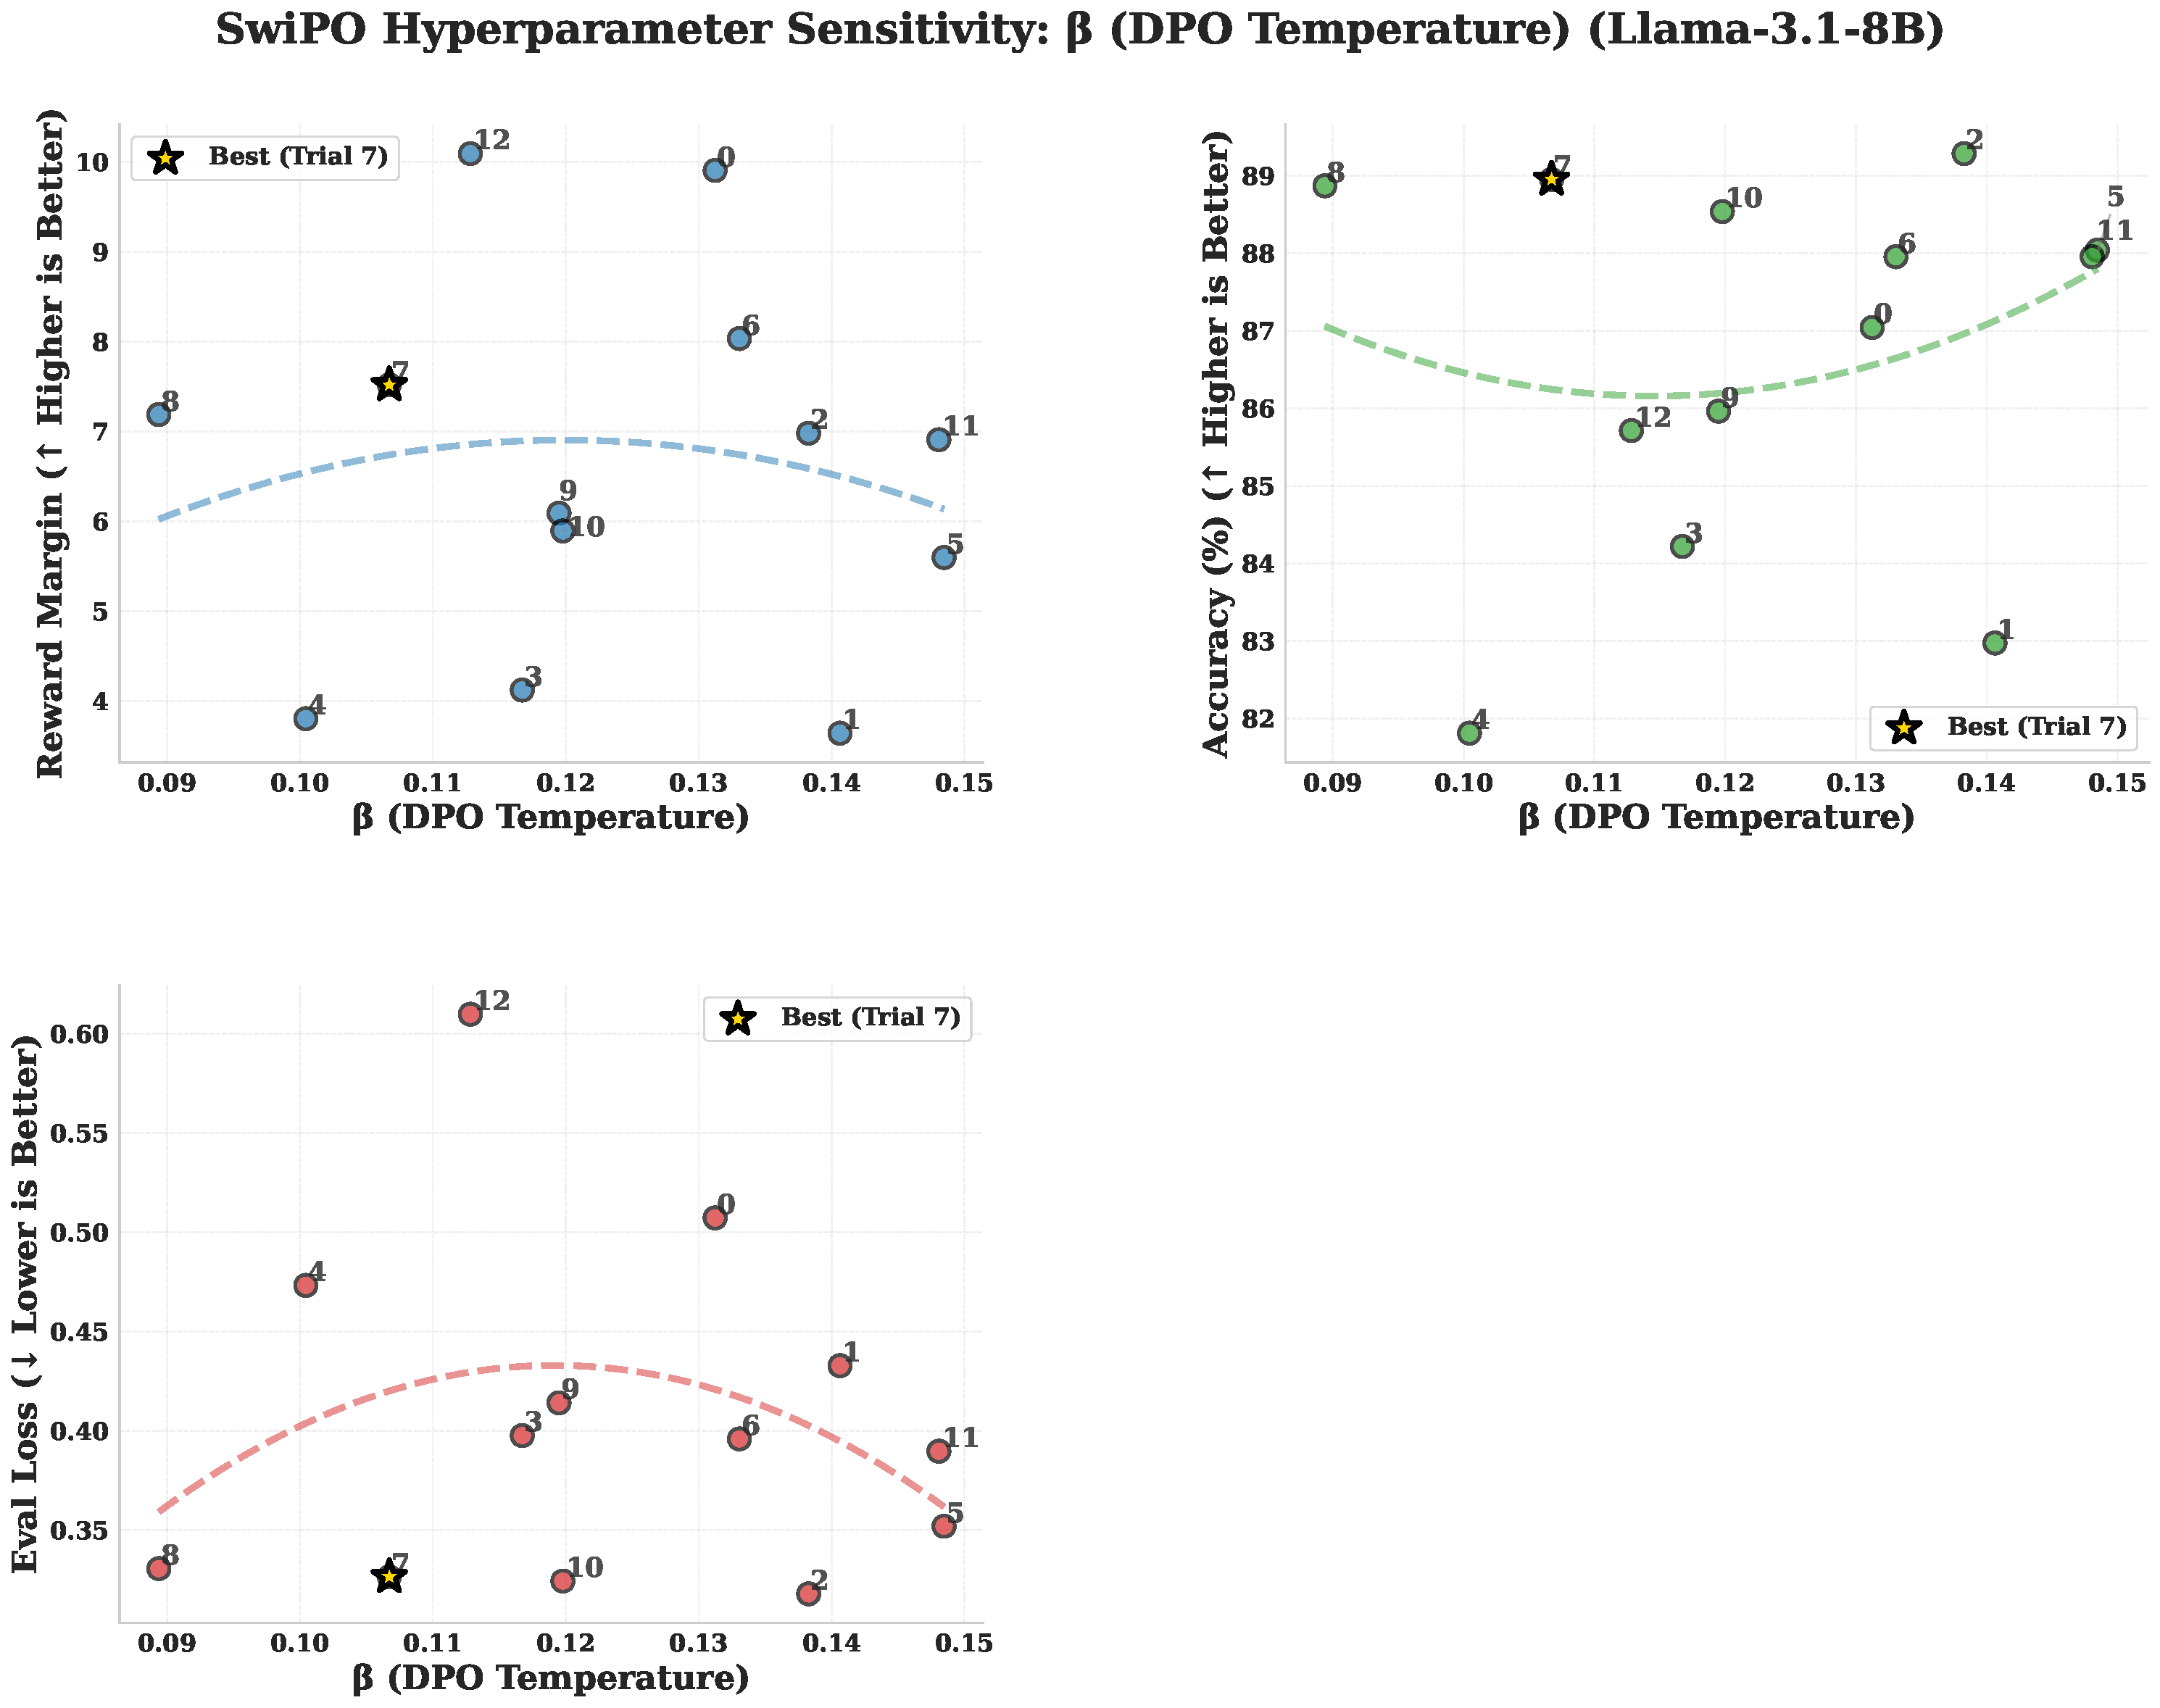
\includegraphics[width=0.85\textwidth]{figures/appendix/hp_ablation_beta.pdf}
\caption{\textbf{$\beta$ sensitivity.} Reward margin peaks at $\beta\approx 0.10$--$0.12$; accuracy is stable (88--90\%), while evaluation loss increases at higher $\beta$, consistent with over-sharpening. Trial 7 ($\star$) at $\beta$=0.107 achieves strong margins while preserving switchability.}
\label{fig:hp_beta}
\end{figure*}

\paragraph{Understanding $\beta$ (DPO temperature).}
Figure~\ref{fig:hp_beta} shows how the DPO temperature parameter $\beta$ affects three training metrics across 13 Optuna trials.
$\beta$ controls the \textbf{sharpness of preference learning}: higher $\beta$ increases the penalty for ranking violations, pushing the model to more decisively separate chosen from rejected responses.
The top-left panel (Reward Margin) reveals a clear \textbf{inverted-U relationship}: margin is low at extreme $\beta$ values and peaks in the 0.10--0.12 range.
At $\beta < 0.10$, preference learning is too soft and the model fails to discriminate strongly; at $\beta > 0.14$, over-sharpening causes the model to collapse toward a single dominant response pattern, destroying multi-regime switching.

\paragraph{$\beta$'s differential effects on metrics.}
The top-right panel (Accuracy) is \textbf{stable} across the $\beta$ range: accuracy varies only from 82\% to 89\%, with no clear trend.
This indicates that $\beta$ primarily affects \textbf{separation magnitude} rather than \textbf{ranking correctness}: the model can correctly rank preferences at any $\beta$, but the confidence of that ranking varies.
The bottom panel (Eval Loss) shows an upward trend: higher $\beta$ increases loss, consistent with the over-sharpening hypothesis.
Trials 0 and 12 achieve very high margins (9.9, 10.1) but also high loss (0.51, 0.61), indicating unstable training.
Trial 7 at $\beta$=0.107 achieves strong margin (7.5) with low loss (0.33), representing the optimal balance.

\begin{figure*}[p]
\centering
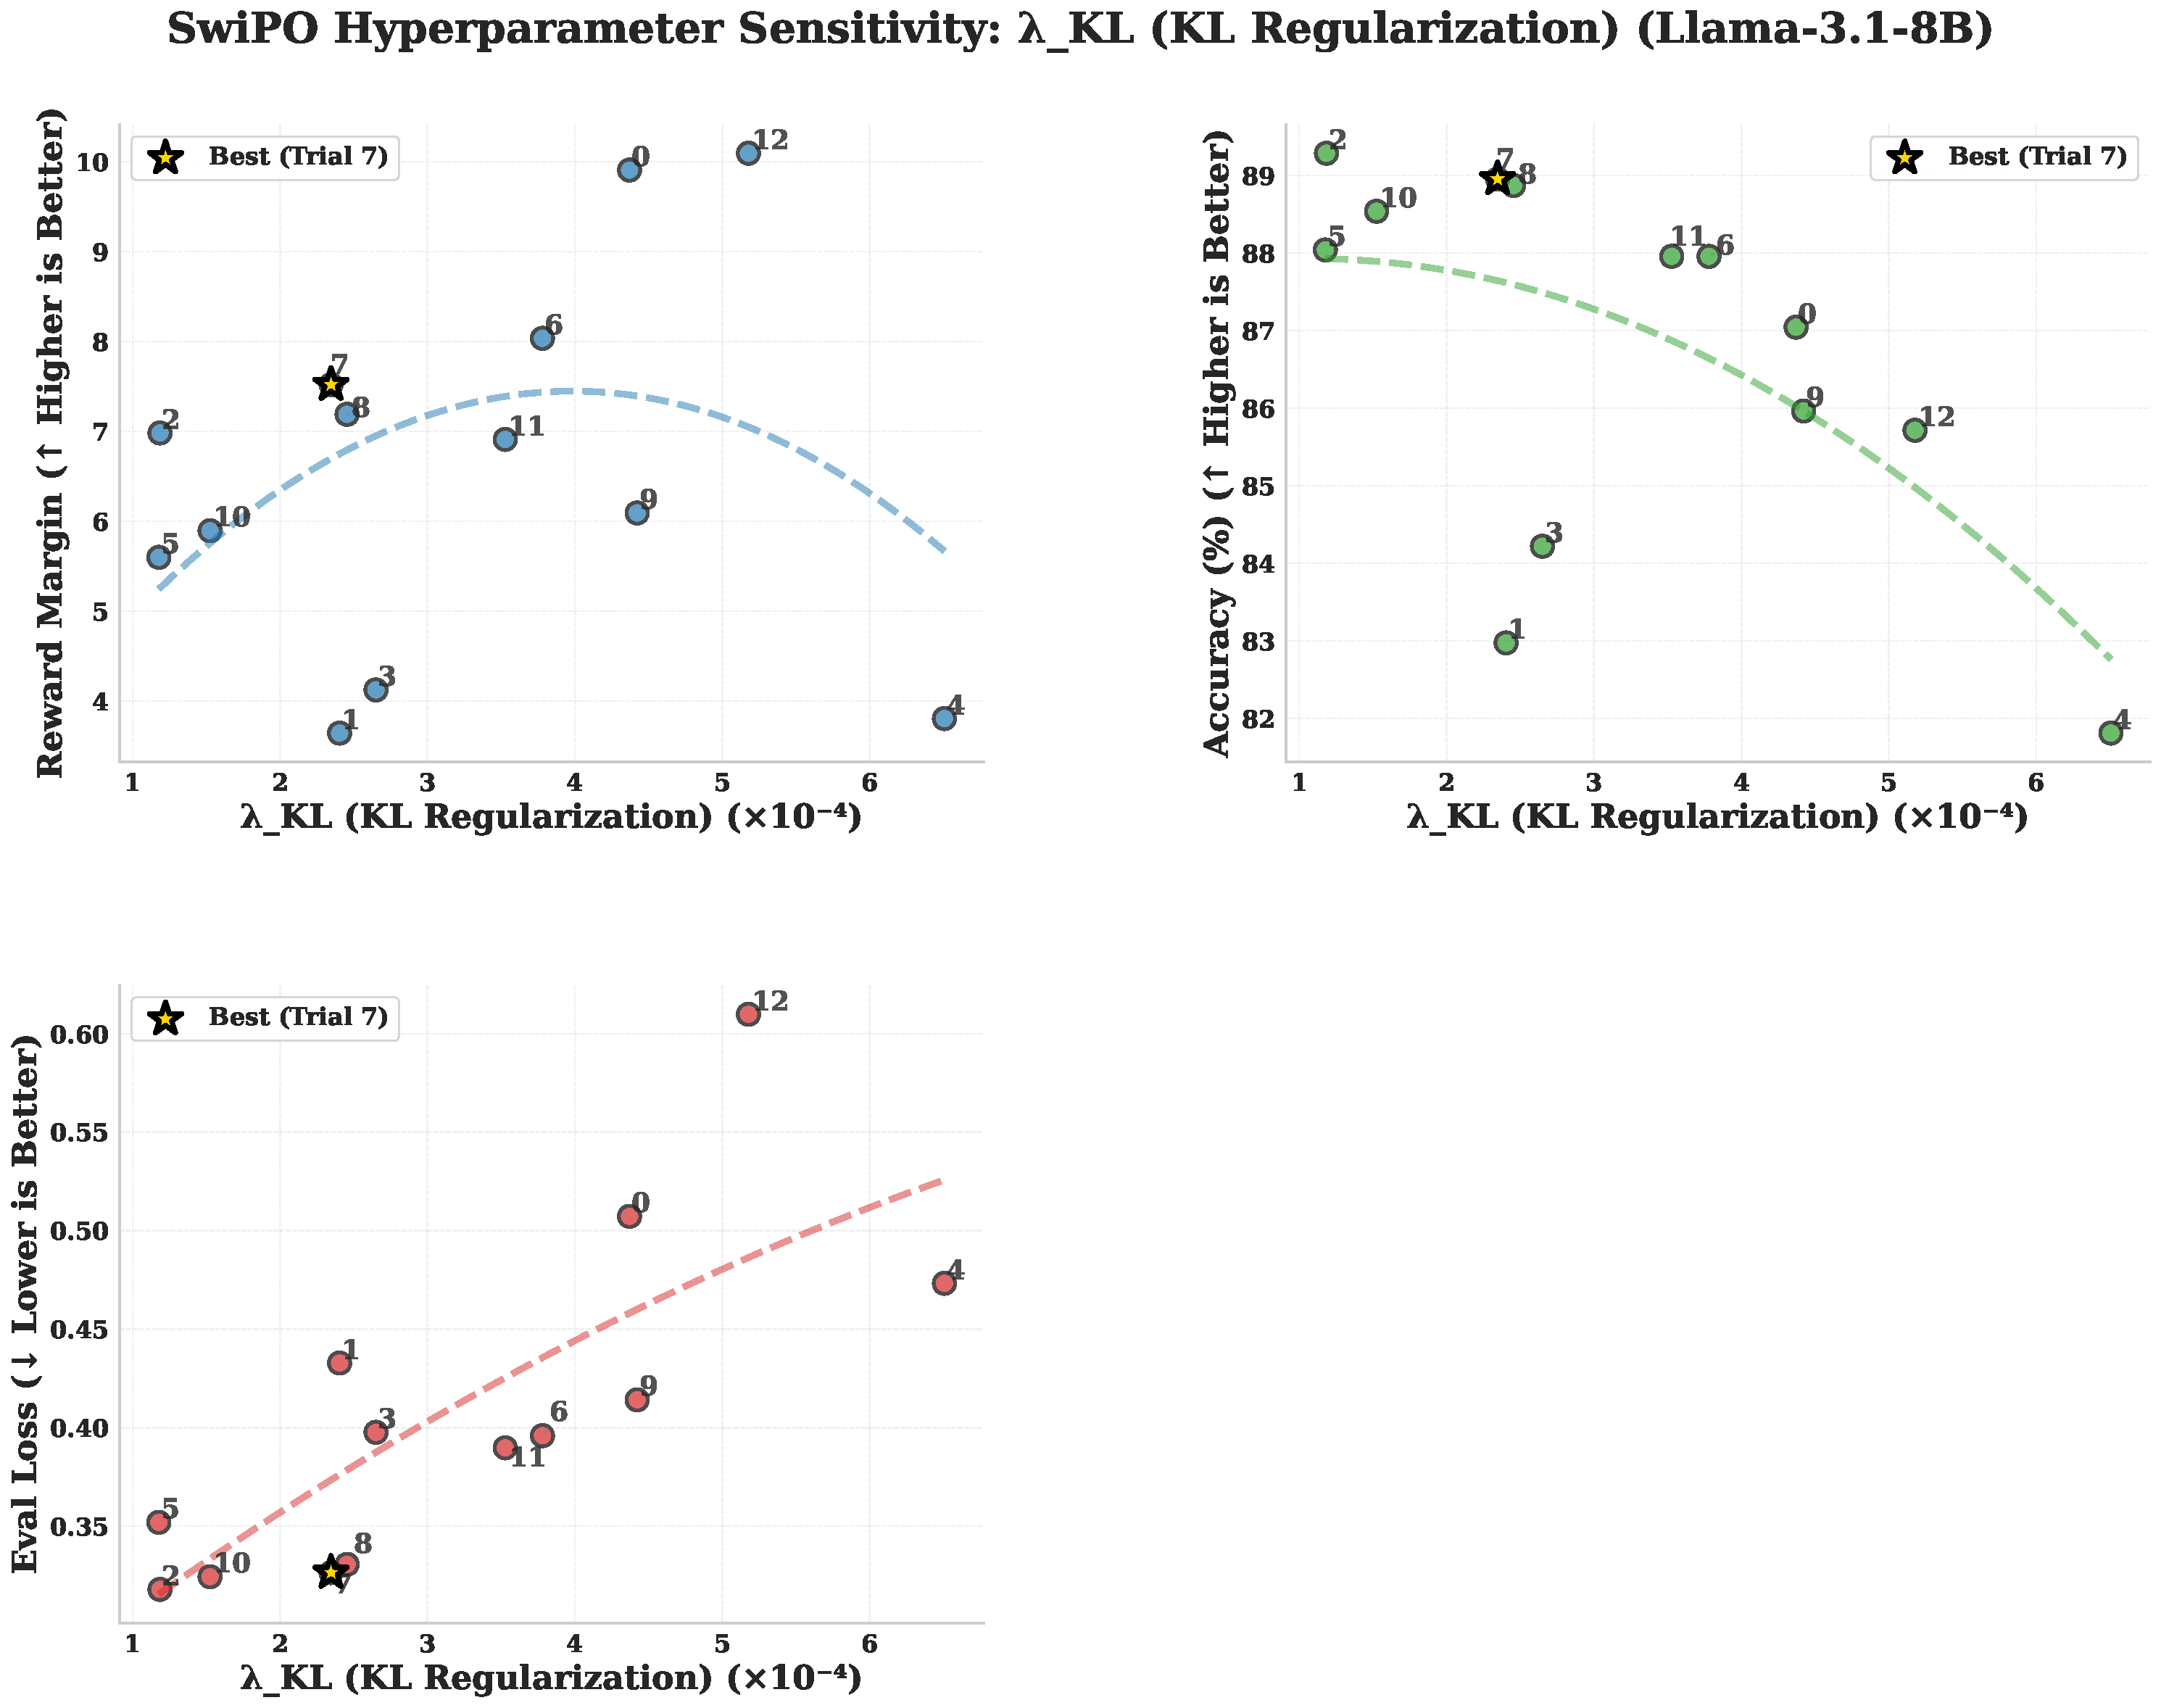
\includegraphics[width=0.85\textwidth]{figures/appendix/hp_ablation_lambda_kl.pdf}
\caption{\textbf{$\lambda_{\text{KL}}$ sensitivity.} Reward margin exhibits an inverted-U: too low produces instability and regime interference; too high suppresses learning. Accuracy is comparatively stable, indicating the dominant effect is on switching stability rather than raw preference fit. Trial 7 ($\star$) at $\lambda_{\text{KL}}$=0.00023 lies in the optimal band.}
\label{fig:hp_lambda}
\end{figure*}

\paragraph{Understanding $\lambda_{\text{KL}}$ (KL regularization).}
Figure~\ref{fig:hp_lambda} shows how the KL regularization coefficient $\lambda_{\text{KL}}$ affects training metrics.
$\lambda_{\text{KL}}$ controls the \textbf{stability anchor} in SwiPO's unified loss: it penalizes deviation from the reference policy (frozen DPO checkpoint), preventing the model from drifting too far during instruction-conditioned training.
The top-left panel (Reward Margin) shows a pronounced \textbf{inverted-U relationship}: margin peaks around $\lambda_{\text{KL}} \approx 2$--$4 \times 10^{-4}$ and drops sharply at both extremes.
Within this search the lowest margins come from the three lowest learning rates (trials 1, 3, and 4), not from the smallest $\lambda_{\text{KL}}$: the two trials with $\lambda_{\text{KL}} < 1.5 \times 10^{-4}$ (trials 2 and 5) reach margins of 6.98 and 5.60.

\paragraph{$\lambda_{\text{KL}}$'s effect on accuracy and loss.}
The top-right panel (Accuracy) shows a \textbf{downward trend}: higher $\lambda_{\text{KL}}$ reduces accuracy from $\sim$89\% to $\sim$82\%.
This is intuitive: stronger KL regularization constrains the policy closer to the reference, limiting its ability to learn new preference patterns and thus reducing ranking accuracy.
The bottom panel (Eval Loss) shows an \textbf{upward trend}: higher $\lambda_{\text{KL}}$ increases loss, reflecting the added KL penalty term in the unified loss.
Trial 7 at $\lambda_{\text{KL}}$=0.00023 achieves the optimal trade-off: strong enough regularization to maintain stability (low loss 0.33) while preserving learning capacity (high accuracy 89\%, margin 7.5).

\paragraph{What this search does not show.}
Whether the anchor is necessary cannot be read from this search: every trial used $\lambda_{\text{KL}}>0$ (the trainer rejects $\lambda_{\text{KL}} \le 0$), and the search space never came close to zero.

\begin{figure*}[ht!]
\centering
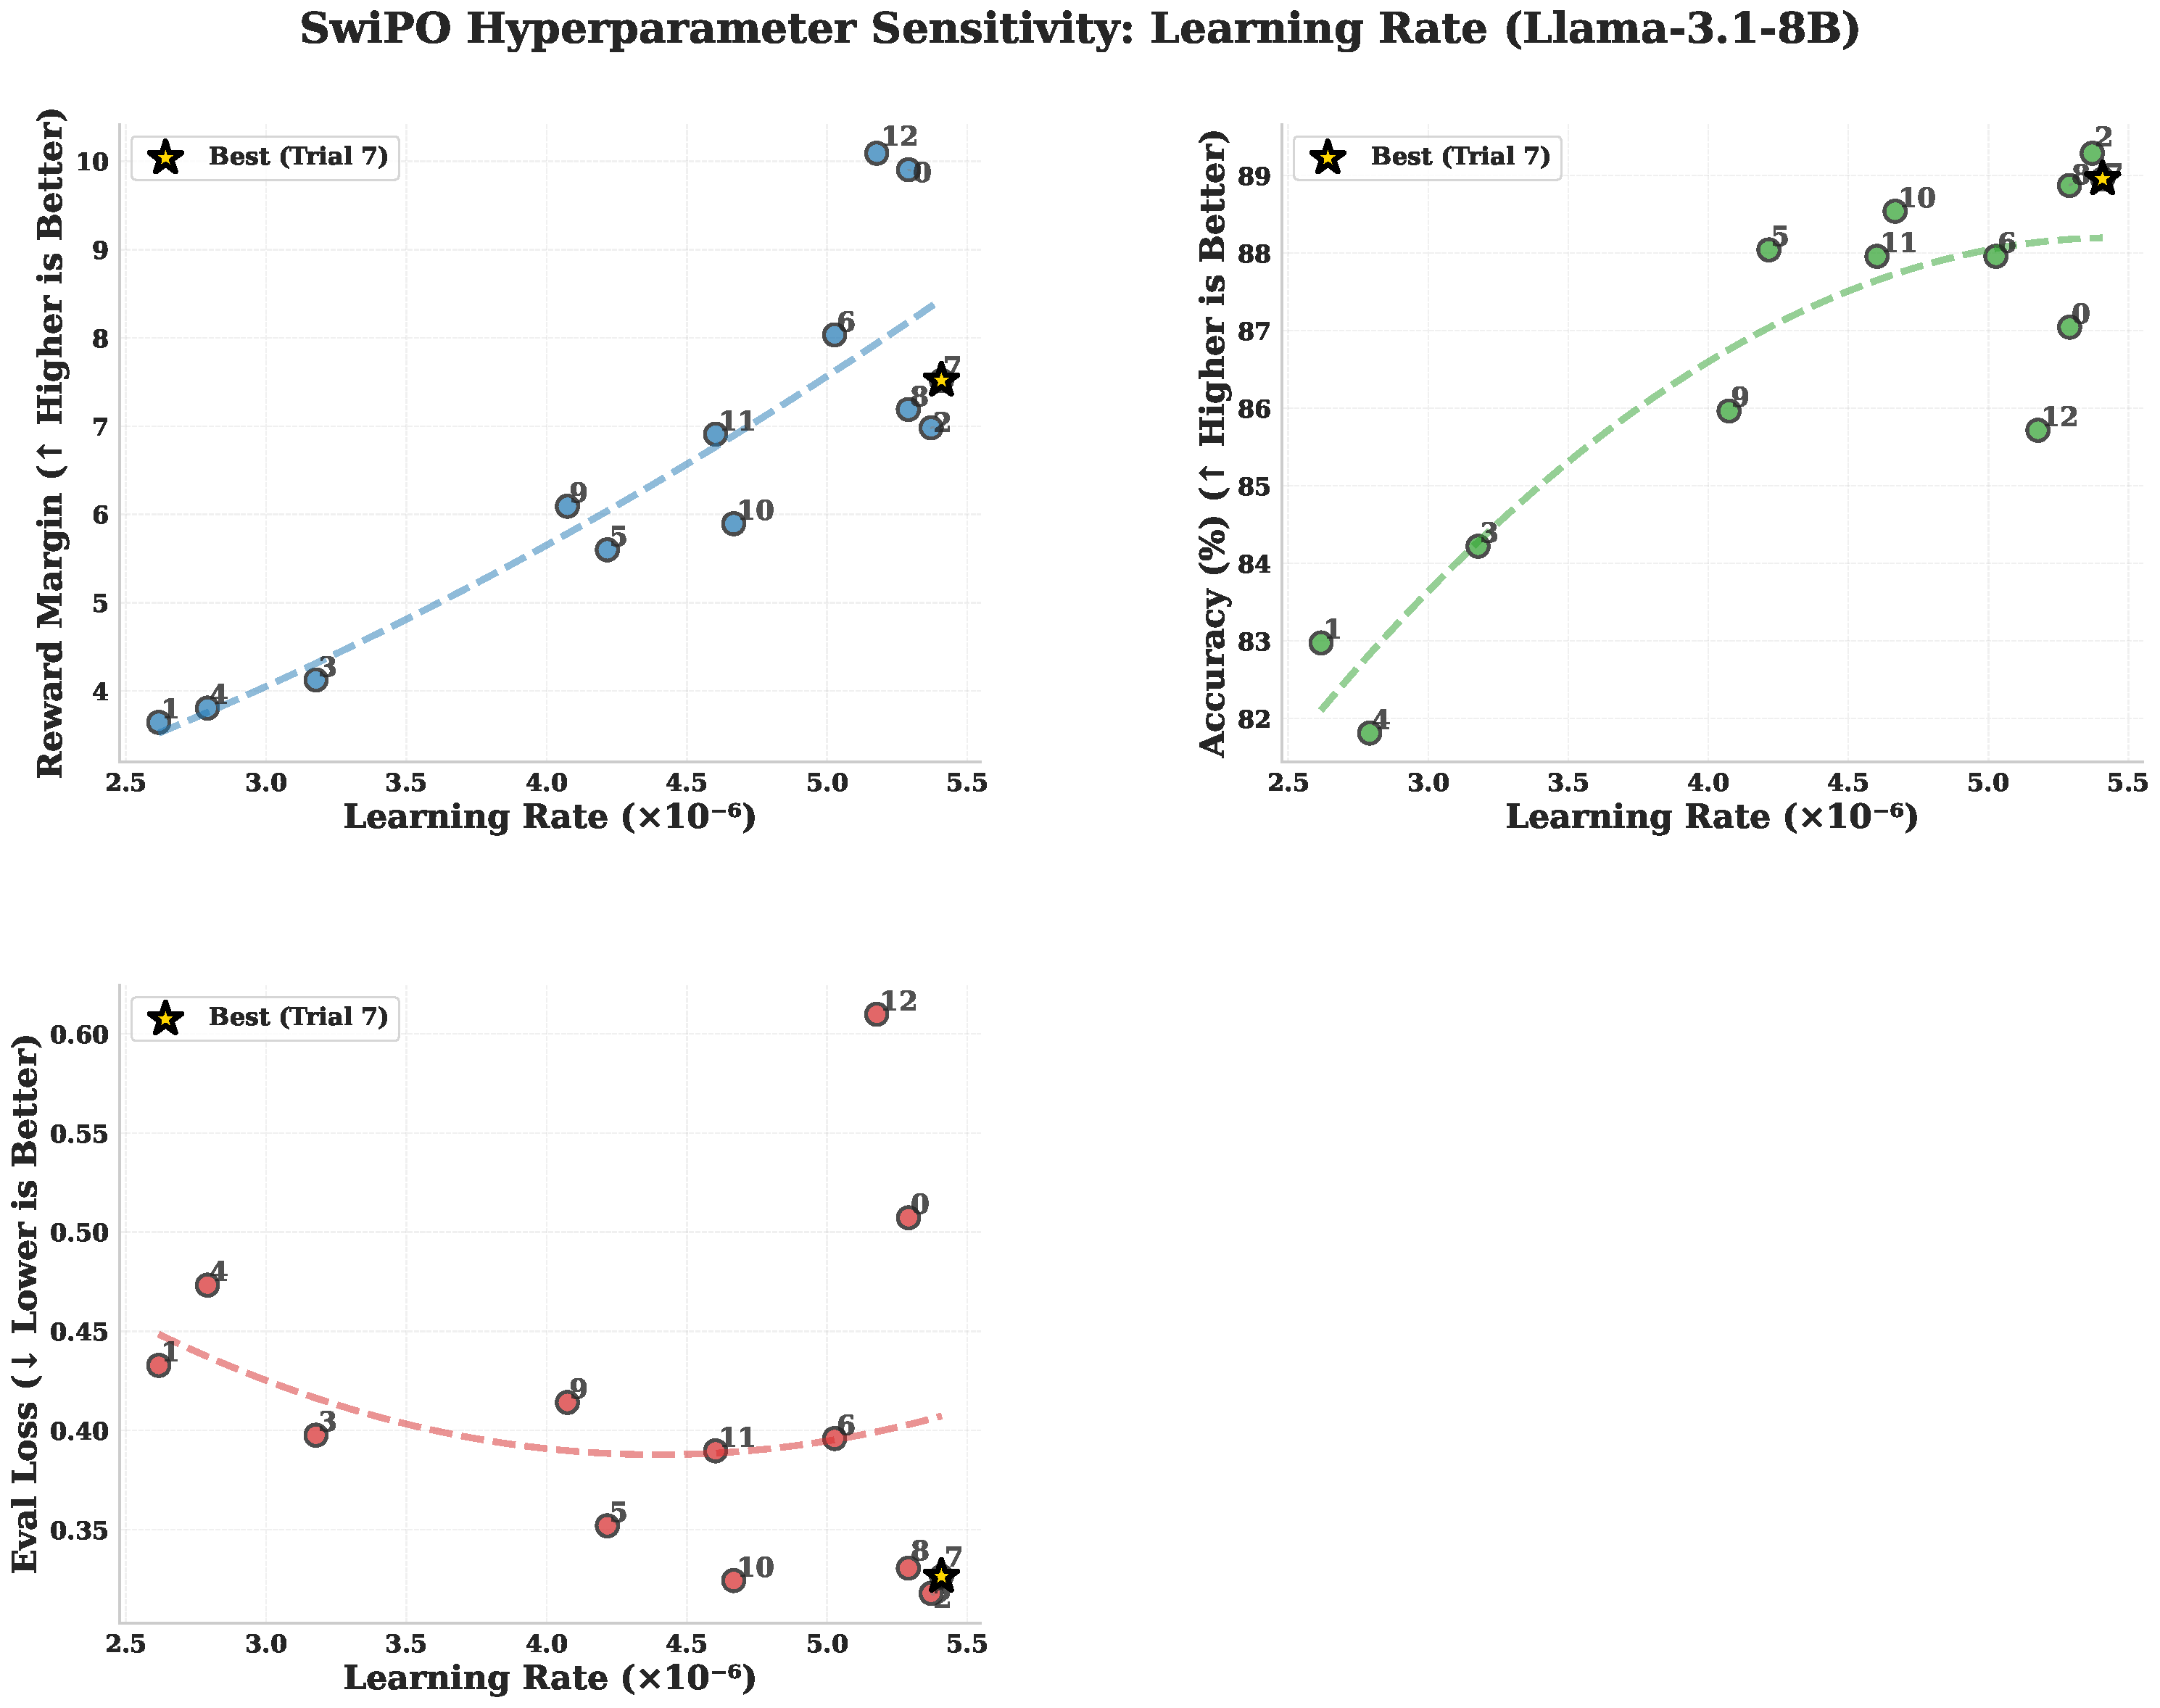
\includegraphics[width=0.9\textwidth]{figures/appendix/hp_ablation_learning_rate.pdf}
\caption{\textbf{Learning-rate sensitivity.} Reward margin is highly sensitive to LR, with an optimum near $5\times 10^{-6}$. Higher LR reduces accuracy and increases loss, especially for instruction-augmented sequences. \textbf{Key insight:} SwiPO\_Instruct requires $\sim$50\% lower LR than standard DPO due to longer contexts and higher gradient variance.}
\label{fig:hp_lr}
\end{figure*}

\paragraph{Learning rate is the dominant sensitivity axis.}
Figure~\ref{fig:hp_lr} reveals that learning rate has the \textbf{strongest effect} on reward margin of any hyperparameter.
The top-left panel shows a clear \textbf{monotonic positive relationship}: margin increases from $\sim$3.5 at LR=$2.5 \times 10^{-6}$ to $\sim$10 at LR=$5.4 \times 10^{-6}$.
This strong correlation (dashed trend line has high $R^2$) indicates that LR directly controls the ``aggressiveness'' of preference learning.
However, the highest-margin trials (0, 12 at LR$\approx$5.2--5.4$\times 10^{-6}$) also exhibit degraded switching on ECLIPTICA, suggesting that very high LR causes over-fitting to preference pairs at the expense of multi-regime flexibility.

\paragraph{LR's effect on accuracy and loss.}
The top-right panel (Accuracy) shows a \textbf{positive correlation}: higher LR improves accuracy from $\sim$82\% to $\sim$89\%.
Unlike $\beta$ and $\lambda_{\text{KL}}$ (where accuracy was relatively stable), LR directly affects how well the model learns to rank preferences correctly.
The bottom panel (Eval Loss) shows a \textbf{U-shaped relationship}: loss is minimized around LR=$4.5$--$5.2 \times 10^{-6}$, increasing at both lower LR (underfitting) and higher LR (overfitting/instability).
Trial 7 at LR=$5.4 \times 10^{-6}$ sits at the edge of the optimal region; slightly higher would risk instability.

\paragraph{Learning rate of SwiPO\_Instruct.}
The selected SwiPO\_Instruct learning rate ($5.4 \times 10^{-6}$) is 21\% below SwiPO\_NoInstruct's ($6.8 \times 10^{-6}$) and 46\% below DPO's ($1 \times 10^{-5}$). The ordering is partly set by the search itself: after an Instruct run at $6.83 \times 10^{-6}$ diverged (loss 214 at 37\% of training), the Instruct space was capped at $[2.5, 5.5] \times 10^{-6}$, while the NoInstruct space stayed at $[5, 8] \times 10^{-6}$. The motivation is that Instruct samples are longer because of the system instruction.

\vspace{-0.25em}
\noindent
\textbf{Overall takeaway.}
The search shows how $\beta$, $\lambda_{\text{KL}}$, and the learning rate trade reward margin against preference accuracy on the training pairs. It does not measure switching, which was evaluated only for the selected configuration.





%% =============================================================================
%% EVALUATION BENEFITS
%% =============================================================================
% =============================================================================
% Appendix: Detailed Evaluation of SwiPO (NeurIPS spotlight; expanded)
% =============================================================================

% Section "Detailed Evaluation of SwiPO" removed 2026-10-20: it reported no measurements and restated the main text.

\section{Training Curves}
\label{sec:appendix_training_curves}

\vspace{-0.25em}
\noindent
This section reports supplementary training dynamics that contextualize the main results in Section~\ref{sec:training_dynamics}.
We emphasize one operational point: \textbf{loss scale is not comparable across methods}.
Offline preference objectives (DPO/SwiPO) and online RL objectives (GRPO) produce different loss magnitudes and noise characteristics.
Accordingly, we interpret curves through \textbf{convergence shape}, \textbf{stability}, and \textbf{relative trends} (Instruct vs.\ NoInstruct), rather than absolute loss values.

\subsection{DPO/SwiPO Eval Loss}

\begin{figure*}[ht!]
\centering
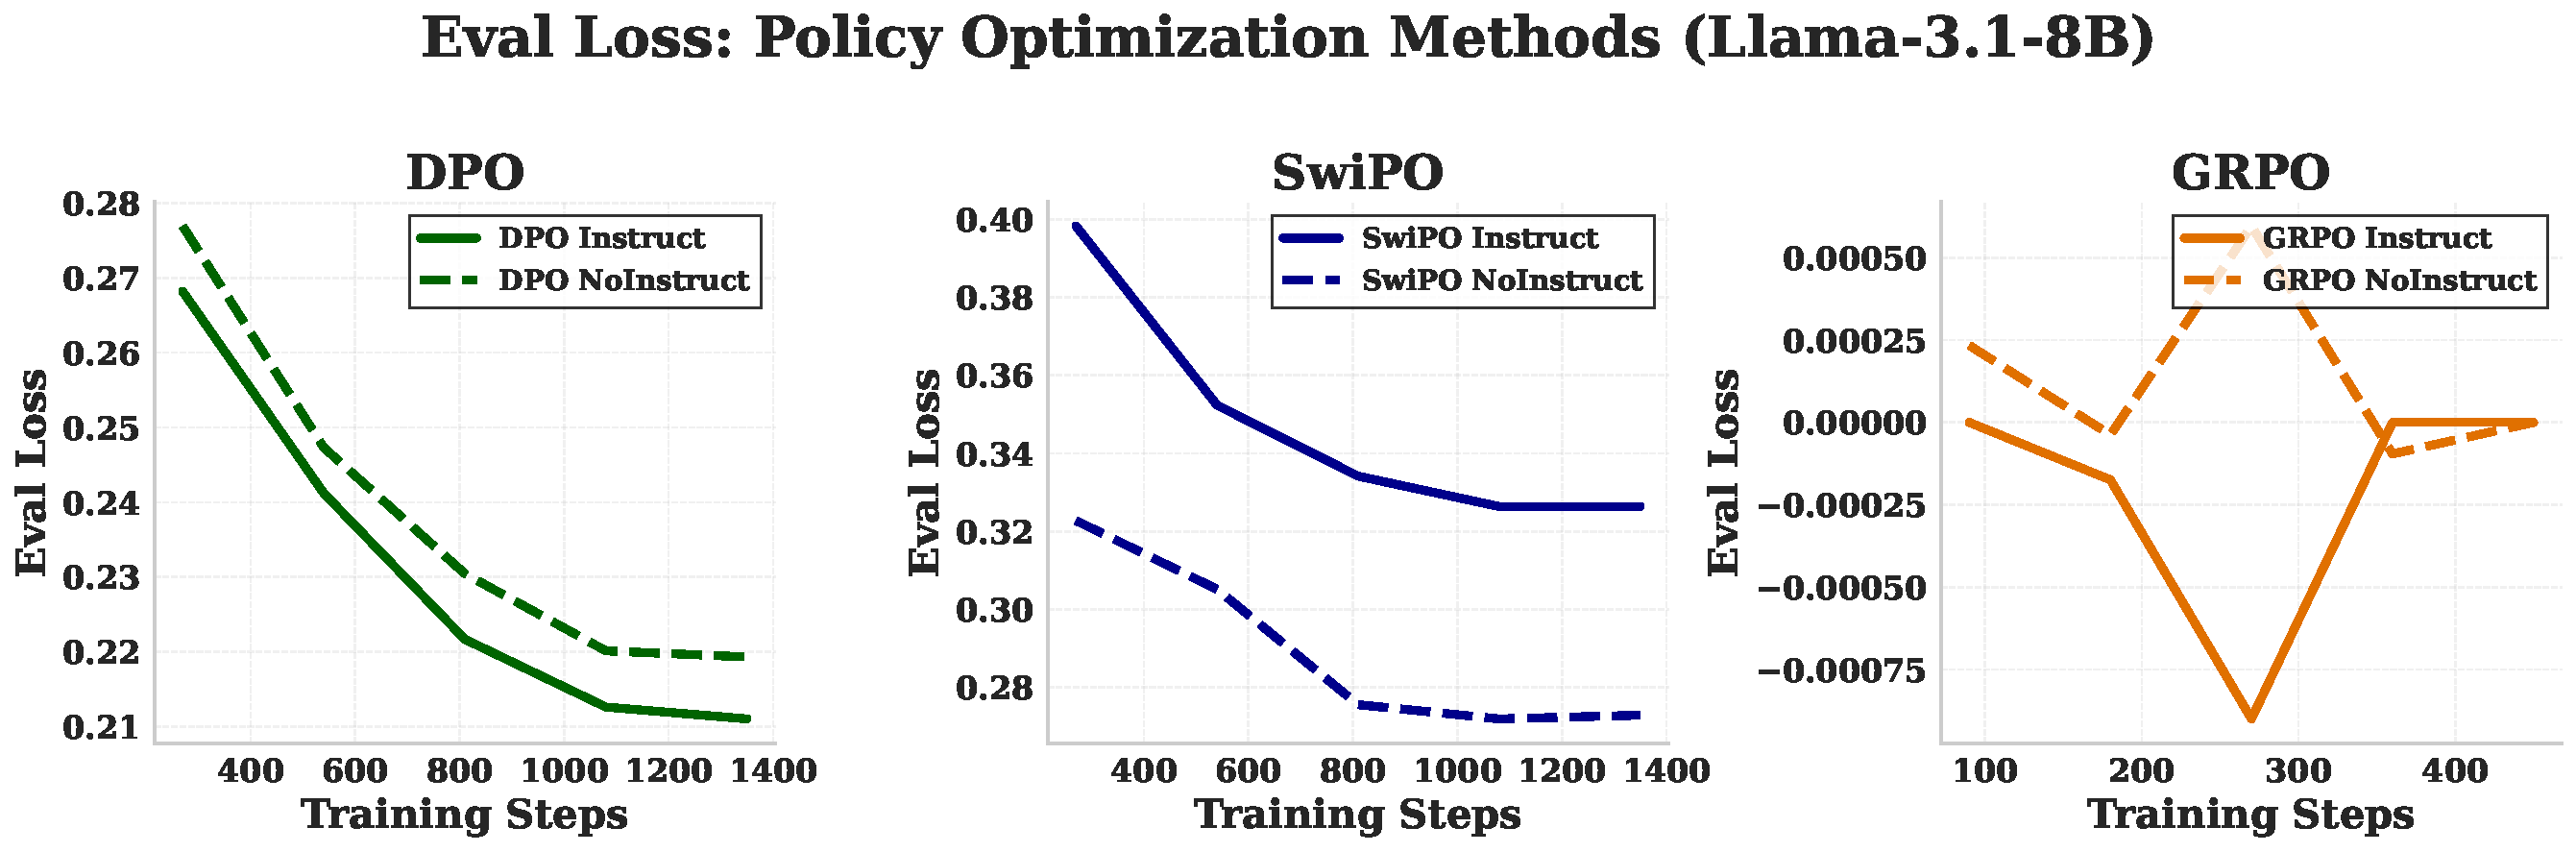
\includegraphics[width=0.9\textwidth]{figures/training/combined_eval_loss.pdf}
\caption{\textbf{Evaluation loss across policy optimization methods.}
We plot evaluation loss for DPO, SwiPO, and GRPO using independent y-axes due to non-comparable loss scales.
\textbf{DPO (left):} loss $\sim$0.21--0.28 with smooth convergence; the Instruct variant is slightly lower, consistent with stronger preference fit under the instruction-augmented setup.
\textbf{SwiPO (center):} loss $\sim$0.27--0.40; the NoInstruct curve converges lower, while SwiPO\_Instruct attains larger reward margins, reflecting a separation--stability trade-off induced by the mandatory anchoring term.
\textbf{GRPO (right):} loss oscillates near zero ($\pm$0.001), characteristic of online RL training where the objective is dominated by on-policy sampling variance.
\textbf{Note:} PPO tensorboard logs were empty due to a TRL logging issue, so we do not include PPO curves here.}
\label{fig:training_loss}
\vspace{-3mm}
\end{figure*}

\vspace{-0.35em}
\noindent\textbf{Key takeaways from Figure~\ref{fig:training_loss}.}
\textbf{First,} DPO exhibits the most stable and smooth offline convergence, serving as a strong baseline for preference fitting.
\textbf{Second,} SwiPO exhibits slightly higher eval loss but achieves higher reward margins, consistent with learning a \textbf{switchable policy family} rather than optimizing a single preference boundary.
\textbf{Third,} GRPO's oscillatory loss highlights the cost of online methods: additional variance and sensitivity to sampling, even when downstream performance can be competitive.

\paragraph{DPO loss dynamics (left panel).}
DPO's evaluation loss decreases monotonically from $\sim$0.28 to $\sim$0.21 over 1,400 training steps, exhibiting textbook offline optimization behavior.
The Instruct variant achieves slightly lower final loss (0.21) compared to NoInstruct (0.22), indicating that instruction-augmented training provides marginally stronger preference signal.
This smooth convergence reflects DPO's core design: by reformulating RLHF as supervised learning on preference pairs, DPO avoids the sampling variance inherent to online methods.
The monotonic decrease also suggests that the learning rate ($1 \times 10^{-5}$) and LoRA configuration (r=16) are well-calibrated for this task.

\paragraph{SwiPO loss dynamics (center panel).}
SwiPO exhibits a different pattern: loss decreases from $\sim$0.40 to $\sim$0.27 (NoInstruct) or $\sim$0.34 (Instruct).
The higher absolute loss compared to DPO is expected because SwiPO's unified loss includes both the DPO term and the KL anchor: $\mathcal{L}_{\mathrm{SwiPO}} = \mathcal{L}_{\text{DPO}} + \lambda_{\text{KL}} \cdot \mathcal{L}_{\text{KL}}$.
The KL term penalizes deviation from the reference policy, which necessarily increases total loss while providing stability benefits.
Notably, SwiPO\_NoInstruct converges to lower loss than SwiPO\_Instruct (the opposite of DPO's pattern) because longer Instruct sequences incur proportionally larger KL penalties.

\paragraph{GRPO loss dynamics (right panel).}
GRPO's loss oscillates near zero ($\pm$0.001), which is characteristic of online RL rather than a sign of instability.
Unlike offline methods that compute loss on a fixed preference dataset, GRPO generates fresh responses at each step and computes group-relative advantages within each batch.
This on-policy sampling introduces inherent variance: different batches of generated responses produce different advantage distributions.
The oscillation around zero reflects that GRPO's loss is a policy gradient objective (expected advantage-weighted log-probability) rather than a supervised loss, making direct magnitude comparisons with DPO/SwiPO inappropriate.
GRPO also runs for fewer steps ($\sim$500) due to the computational overhead of online generation.

\paragraph{Why PPO curves are absent.}
PPO tensorboard logs were empty due to a known TRL logging issue where the PPOTrainer's internal metrics are not properly exported to tensorboard in certain configurations.
Despite the missing training curves, PPO evaluation results (Section~\ref{sec:overall_results}) confirm that PPO training completed successfully and produced competitive models, particularly on the AQI benchmark where PPO's online optimization shapes global reward-aligned behavior.


